\documentclass[11pt,a4paper]{article}

\usepackage[utf8]{inputenc}
\usepackage[T1]{fontenc}
\usepackage[brazil]{babel}
\usepackage{lmodern}
\usepackage{helvet}
\renewcommand{\familydefault}{\sfdefault}
\usepackage{amssymb}
\usepackage[margin=2.5cm]{geometry}
\usepackage[table]{xcolor}
\usepackage{titlesec}
\usepackage{tabularx}
\usepackage{booktabs}
\usepackage{array}
\usepackage{enumitem}
\usepackage{fancyvrb}
\usepackage{tikz}
\usetikzlibrary{positioning}
\usepackage{graphicx}
\usepackage[hidelinks]{hyperref}

% ----------------------------------------------------------------------------
% Paleta minimalista: cinza + off-white ("branco escuro")
% ----------------------------------------------------------------------------
\definecolor{pagebg}{HTML}{F3F2F0}   % fundo off-white
\definecolor{ink}{HTML}{2E2E2E}       % texto (cinza bem escuro)
\definecolor{headgray}{HTML}{4A4A4A}  % títulos
\definecolor{rulegray}{HTML}{C9C7C3}  % linhas finas
\definecolor{boxbg}{HTML}{E9E8E5}     % caixas/código
\definecolor{accent}{HTML}{7C7C7C}    % detalhes

\pagecolor{pagebg}
\color{ink}

\setlength{\emergencystretch}{3em}
\setlength{\parindent}{0pt}
\setlength{\parskip}{6pt}

% Títulos minimalistas com filete fino
\titleformat{\section}
  {\color{headgray}\Large\bfseries}{\thesection}{0.6em}{}[{\color{rulegray}\titlerule[0.6pt]}]
\titleformat{\subsection}
  {\color{headgray}\large\bfseries}{\thesubsection}{0.5em}{}
\titlespacing*{\section}{0pt}{14pt}{6pt}

\newcolumntype{Y}{>{\raggedright\arraybackslash}X}

% Tabela com cabeçalho em cinza claro
\newcommand{\headrow}[1]{\rowcolor{boxbg}#1}

\newcommand{\done}{{\color{headgray}$\boxtimes$}}
\newcommand{\todo}{{\color{accent}$\square$}}

\begin{document}

% ----------------------------------------------------------------------------
% Capa minimalista
% ----------------------------------------------------------------------------
\thispagestyle{empty}
\vspace*{1cm}
{\color{rulegray}\rule{\textwidth}{0.6pt}}\\[10pt]
{\color{headgray}\fontsize{26}{30}\selectfont\bfseries Gestão de Equipamentos}\\[6pt]
{\color{accent}\large API REST em .NET --- Trabalho Final do Módulo 3 (Desenvolvimento em C\#)}\\[10pt]
{\color{rulegray}\rule{\textwidth}{0.6pt}}

\vspace{4pt}
{\color{accent}\small Documento de planejamento e status do projeto.}

\vspace{18pt}

\section{Resumo do projeto}

Sistema de \textbf{Gestão de Equipamentos}: cadastro de equipamentos, categorias,
localização (fornecedores), histórico de manutenções/ações e usuários. API REST em
ASP.NET Core, persistência em PostgreSQL via Entity Framework Core, arquitetura em
camadas (API, Application, Domain, Infrastructure, Exceptions).

\section{Modelo de dados}

Esquema gerado pelas entidades + migrations do EF Core e verificado no PostgreSQL.
Relacionamentos por chave estrangeira em destaque.

\vspace{4pt}
\begin{center}
\begin{tikzpicture}[
  every node/.style={font=\scriptsize},
  tbl/.style={draw=rulegray, line width=0.5pt, rounded corners=3pt, fill=white,
              text=ink, align=left, inner sep=6pt},
  fk/.style={draw=accent, line width=0.8pt},
  lbl/.style={font=\scriptsize\itshape, text=accent, fill=pagebg, inner sep=1pt}
]
  \node[tbl] (eq) {\textbf{Equipments}\\[2pt]
    Id (PK)\\ Name\\ SerialNumber\\ Model\\ PurchaseDate\\ Status\\
    CategoryId (FK)\\ SupplierId (FK)};

  \node[tbl, right=2.6cm of eq, yshift=2.1cm] (cat) {\textbf{Categories}\\[2pt] Id (PK)\\ Name};
  \node[tbl, right=2.6cm of eq, yshift=-2.1cm] (sup) {\textbf{Suppliers}\\[2pt] Id (PK)\\ Name\\ ContactEmail};
  \node[tbl, left=2.6cm of eq] (hist) {\textbf{EquipmentHistories}\\[2pt] Id (PK)\\ EquipmentId (FK)\\ Action\\ CreatedAt};
  \node[tbl, below=1.6cm of eq] (usr) {\textbf{Users}\\[2pt] Id (PK)\\ Name\\ Email\\ PasswordHash};

  \draw[fk] (eq.east) -- node[lbl]{N\,:\,1} (cat.west);
  \draw[fk] (eq.east) -- node[lbl]{N\,:\,1} (sup.west);
  \draw[fk] (hist.east) -- node[lbl]{N\,:\,1} (eq.west);
\end{tikzpicture}
\end{center}

\begin{center}
{\color{accent}\scriptsize Users ainda sem relacionamento (entra com a autenticação).}
\end{center}

\subsection*{Entidades}

\begin{tabularx}{\textwidth}{@{}l Y@{}}
\toprule
\headrow{\textbf{Entidade} & \textbf{Descrição}} \\
\midrule
\textbf{Equipment} & Item gerenciado; liga-se a Category e Supplier. \\
\textbf{Category} & Classificação do equipamento (nome único). \\
\textbf{Supplier} & Fornecedor (nome e e-mail de contato). \\
\textbf{EquipmentHistory} & Histórico de ações de um equipamento. \\
\textbf{User} & Usuário do sistema (login/senha) --- usado na autenticação. \\
\bottomrule
\end{tabularx}

\section{Arquitetura em camadas}

\begin{Verbatim}[frame=single, framerule=0.5pt, rulecolor=\color{rulegray}, fontsize=\footnotesize]
Cliente / Swagger / Postman
    |
GestaoEquipamentos.API             controllers, Swagger, auth, Program.cs
GestaoEquipamentos.Application      DTOs, services, interfaces, casos de uso
GestaoEquipamentos.Domain           entidades, enums, regras essenciais
GestaoEquipamentos.Infrastructure   DbContext, repositories, configurations, migrations
    |
PostgreSQL
\end{Verbatim}

A camada Domain não referencia EF Core nem infraestrutura. Exceptions é transversal
(exceções customizadas e padronização de erros).

\section{Divisão de tarefas}

\begin{tabularx}{\textwidth}{@{}l l Y@{}}
\toprule
\headrow{\textbf{Camada / Tema} & \textbf{Responsável} & \textbf{Status}} \\
\midrule
\textbf{Infrastructure} & Camila & \done\ Concluída (repositórios, DbSets, configurations, migrations). \\
\textbf{Domain} & Lucas & \done\ Entidades e enums criados. \\
\textbf{API} & Lucas / Pedro & \todo\ Controllers, Swagger, middlewares, wiring. \\
\textbf{Application} & Paulo & \todo\ DTOs, services e validações em andamento. \\
\textbf{Exceptions} & Adriano & \todo\ Exceções e middleware global de erro. \\
\textbf{Autenticação} & Pedro & \todo\ Registro/login, hash de senha, JWT. \\
\bottomrule
\end{tabularx}

\section{Camada Infrastructure --- entregue}

\begin{itemize}[leftmargin=1.2em, itemsep=2pt]
  \item \textbf{Repositório genérico} \texttt{Repository<T>} + \texttt{IRepository<T>} (CRUD reutilizável).
  \item \textbf{Repositórios específicos:} Equipment (com filtro por categoria), Category,
        Supplier e EquipmentHistory (com filtro por equipamento).
  \item \textbf{DbContext} com os \texttt{DbSet} de todas as entidades e aplicação automática
        das configurations (\texttt{ApplyConfigurationsFromAssembly}).
  \item \textbf{Configurations} (\texttt{IEntityTypeConfiguration}): tamanhos de campo,
        índice único (Category.Name, Equipment.SerialNumber), tipo \texttt{date} e a
        chave estrangeira EquipmentHistory $\rightarrow$ Equipment.
  \item \textbf{Injeção de dependência:} \texttt{AddInfrastructure} registra o DbContext
        (Npgsql/PostgreSQL) e todos os repositórios.
  \item \textbf{Banco:} PostgreSQL em container (porta 5433), connection string configurada.
\end{itemize}

\section{Artefatos}

\subsection*{Migrations aplicadas}

\begin{tabularx}{\textwidth}{@{}l Y@{}}
\toprule
\headrow{\textbf{Migration} & \textbf{O que faz}} \\
\midrule
\texttt{InitialCreate} & Cria todas as tabelas a partir das entidades. \\
\texttt{ConfigureEquipment} & Tamanhos de campo, serial único e \texttt{PurchaseDate} como date. \\
\texttt{ConfigureRemainingEntities} & Regras de Category, Supplier e EquipmentHistory. \\
\texttt{AddEquipmentHistoryForeignKey} & FK EquipmentHistory $\rightarrow$ Equipment. \\
\bottomrule
\end{tabularx}

\subsection*{Como rodar (resumo)}

\begin{Verbatim}[frame=single, framerule=0.5pt, rulecolor=\color{rulegray}, fontsize=\footnotesize]
docker compose up -d
dotnet ef database update --project GestaoEquipamentos.Infrastructure
dotnet run --project GestaoEquipamentos.API
\end{Verbatim}

\section{Evidências (PostgreSQL via DBeaver)}

Banco \texttt{gestao\_equipamentos} inspecionado no DBeaver após aplicar as migrations.

\begin{center}
\fcolorbox{rulegray}{white}{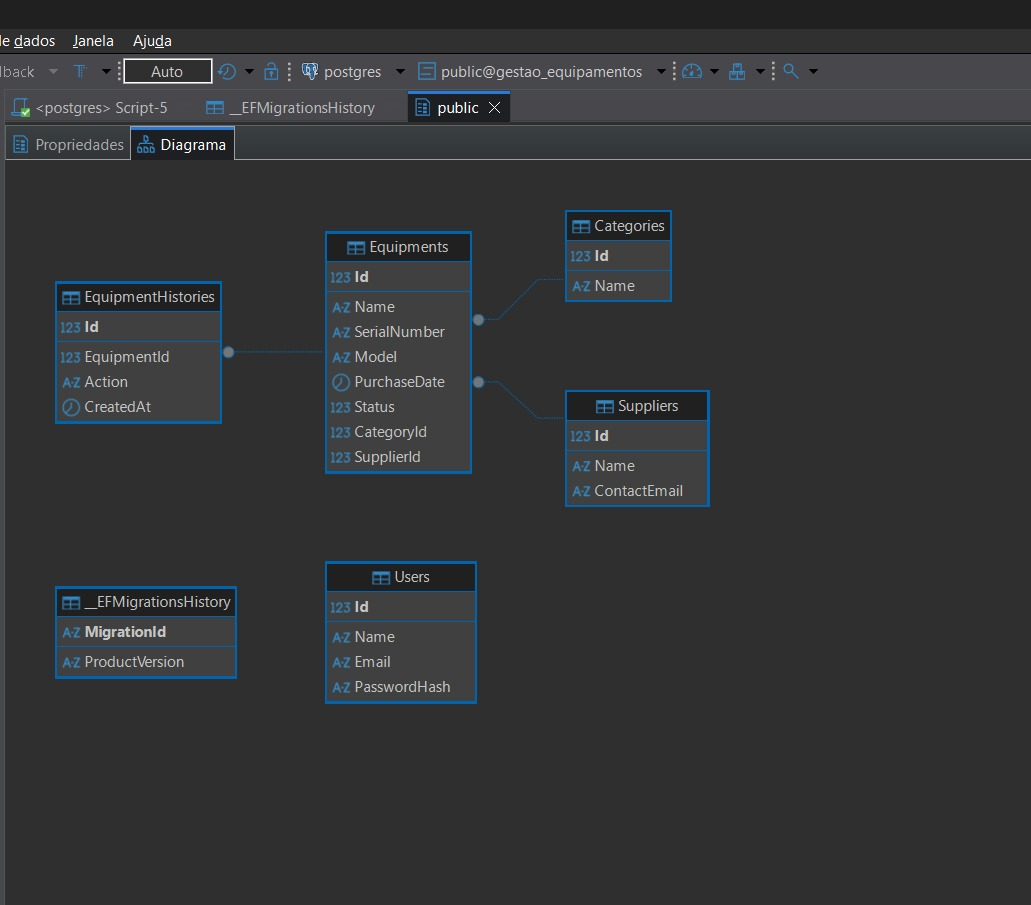
\includegraphics[width=0.92\textwidth]{artefatos/diagrama-er.jpeg}}\\[3pt]
{\color{accent}\scriptsize Diagrama ER --- relacionamentos Equipment--Category, Equipment--Supplier e EquipmentHistory--Equipment.}
\end{center}

\begin{center}
\fcolorbox{rulegray}{white}{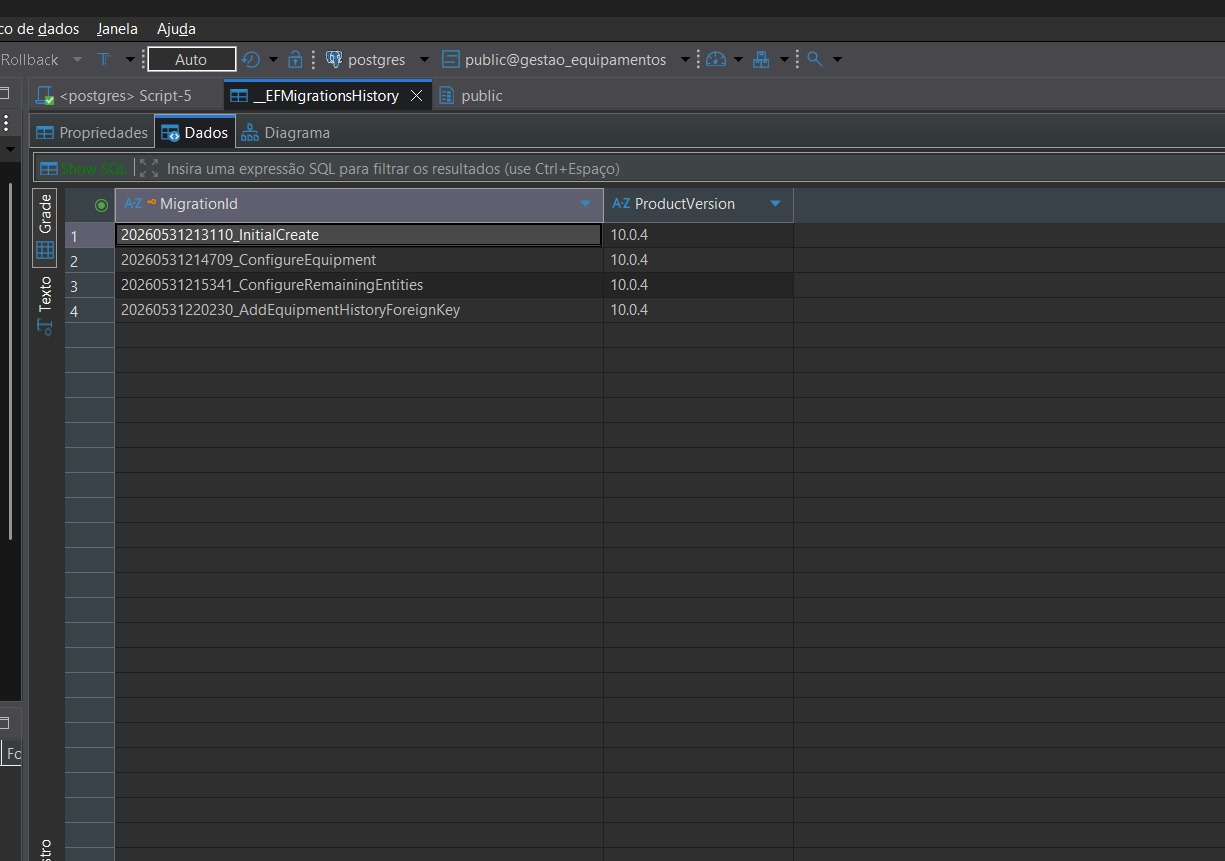
\includegraphics[width=0.92\textwidth]{artefatos/migrations.jpeg}}\\[3pt]
{\color{accent}\scriptsize Tabela \texttt{\_\_EFMigrationsHistory} --- as 4 migrations aplicadas no banco.}
\end{center}

\begin{center}
\fcolorbox{rulegray}{white}{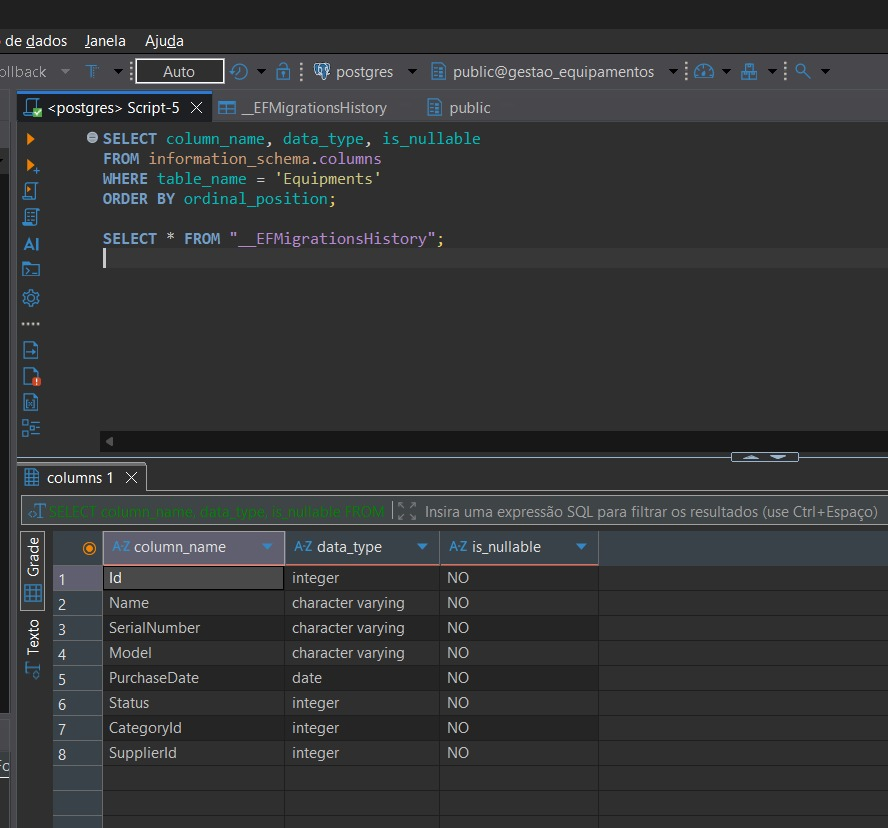
\includegraphics[width=0.85\textwidth]{artefatos/colunas-equipments.jpeg}}\\[3pt]
{\color{accent}\scriptsize Colunas da tabela \texttt{Equipments} --- tipos aplicados pela configuration (varchar, date).}
\end{center}

\section{Checklist do professor}

\begin{tabularx}{\textwidth}{@{}c Y c Y@{}}
\done & PostgreSQL como banco        & \done & EF Core com provider Npgsql \\
\done & Solução em 5 projetos        & \done & Acesso a dados na Infrastructure \\
\done & Migrations entregues         & \done & Relacionamentos entre entidades \\
\done & Repositório Git              & \todo & Autenticação (JWT) \\
\todo & DTOs de entrada/saída        & \todo & Regras de negócio em services \\
\todo & Swagger habilitado           & \todo & Endpoints (auth, CRUD, filtros) \\
\end{tabularx}

\vspace{10pt}
{\color{rulegray}\rule{\textwidth}{0.6pt}}\\[2pt]
{\color{accent}\scriptsize Legenda: \done\ concluído \quad \todo\ pendente.}

\end{document}
